% version 1.01	Auteur Pierre Porche

\section{Mise en place et amélioration de la qualité}\label{qualite}

\subsection{Précisions}
\label{Precisions}
Le client, \nomClient , souhaite que l’équipe \nomEquipe{} utilise les méthodes de travail de son choix pour
la gestion de projet. Cette dernière a donc choisi la méthode en spirale qui sera donc adaptée au suivi de la qualité demandé par l’Unité P3.

\subsection{Objectifs Qualité}
\label{Objectifs qualite}
\paragraph*{} L’objectif de ce projet est d’avoir un bon fonctionnement du PIC tout au long de sa durée et de satisfaire le client par rapport aux résultats fournis. Afin d’améliorer le \SMQ , des objectifs ont été établis par \nomEquipe .
\paragraph*{} Pour garantir la satisfaction du client, nous estimons que nous devrons assurer plusieurs
sous-objectifs :
\begin{itemize} 
          \item L’avancement du projet ;
          \item Le respect des délais ;
          \item La conformité des produits ;
	\item L’efficience du traitement des \FT ;
	\item Une bonne communication.
	
 \end{itemize}
\paragraph*{} Un autre objectif très important est d’assurer la satisfaction de l’Unité P3 au sens de
la gestion du projet et du management de la qualité au sein du PIC. Pour bien suivre et
améliorer cet objectif, nous utiliserons les indicateurs détaillés dans la partie 6.1.4.


\subsection{Évolution du Système de Management de la Qualité}
\label{Evolution du systeme de management de la qualite}

\paragraph*{} La politique qualité du PIC \nomEquipe{} mise en place, sera suivie et corrigée tout au long
du projet par le \RQ . Tout document lié à la qualité rédigé par \nomEquipe,
comme le \PQ{} ou le \PGC , sera mis à jour régulièrement.
\paragraph*{} Le tutorat Qualité permet aux membres du PIC et tout particulièrement au \CP, au
\RQ{} et au \RGC , d’avoir un interlocuteur
compétent dans le domaine de la Qualité. Des réunions fréquentes auront lieu avec le
Tuteur Qualité. Pendant cette réunion, des questions sur le \SMQ{} et sur les différents documents à produire par l’équipe PIC pourront être posées.
Cette réunion permettra ainsi d’améliorer la qualité au sein du PIC.


\subsection{Indicateurs}
\label{Indicateurs}
\subsubsection*{Rôle des indicateurs}
\label{Role des indicateurs}

\paragraph*{} Des indicateurs ont été mis en place par l'équipe \nomEquipe{} dans le but d'assurer le suivi
de la qualité tout au long du PIC. Ils permettront de mesurer et d'évaluer la progression de
l'équipe conformément aux objectifs qualité fixés précédemment.

\paragraph*{} Ces indicateurs seront mis à jour par le \RQ{} puis diffusés, après chaque
mise à jour, à l'ensemble de l'équipe \nomEquipe .

\paragraph*{} Ces indicateurs peuvent être classés selon deux catégories :
\begin{itemize} 
	\item les indicateurs hebdomadaires ;
	\item les indicateurs ponctuels.
 \end{itemize}

\subsubsection*{Indicateurs hebdomadaires}
\label{Indicateurs hebdomadaires}
\paragraph*{} Les indicateurs hebdomadaires permettent de décrire les résultats hebdomadaires en terme
d'avancement du projet, d'efficacité de la communication et de respect du Système de Management de la Qualité.

\paragraph*{} Un tableau récapitulant les indicateurs hebdomadaires mis en place est disponible dans le
tableau 6.1. Pour les indicateurs faisant référence à des délais, le comptage exclut les vacances
scolaires, les jours fériés ainsi que les cours obligatoires sur les créneaux de PIC.


\begin{table}[H]

\begin{tabular}[h]{|p{0.35\textwidth}|p{0.35\textwidth}|p{0.2\textwidth}|}
	\hline
	\rowcolor[gray]{0.85}
	Indicateurs & Valeur cible & Valeur seuil \\\hline
	\multicolumn{3}{|c|}{Processus-Objectif} \\\hline
	\multicolumn{3}{|c|}{\cellcolor[gray]{0.85} Gestion de Projet} \\
	\multicolumn{3}{|c|}{\cellcolor[gray]{0.85} Assurer l'avancement du projet et le respect des délais} \\\hline
	Volume horaire insuffisant & 27h (CP \& RQ) & 22h (CP \& RQ)  \\
	 & 22h (autres) & 17h (autres)  \\\hline
	Retard de tâches & 0\% & 30\% \\\hline
	\multicolumn{3}{|c|}{\cellcolor[gray]{0.85} Gestion de Projet} \\
	\multicolumn{3}{|c|}{\cellcolor[gray]{0.85} Assurer une bonne communication} \\\hline
	Délai entre la tenue de la réunion et l'émission du CR & 4 jours & 7 jours \\\hline
	\multicolumn{3}{|c|}{\cellcolor[gray]{0.85} Management de la qualité} \\
	\multicolumn{3}{|c|}{\cellcolor[gray]{0.85} Assurer un bon système de gestion de la qualité} \\\hline
	Délai entre la date de correction de FT annoncé et la date réelle & 0 jours & 7 jours d'écart \\\hline
	\multicolumn{3}{|c|}{\cellcolor[gray]{0.85} Veille à la qualité du code} \\
	Taux de duplication du code & 5 \% & 15 \% \\\hline
	Nombre de bug & 0 & 3 \\\hline
	
\end{tabular}
\caption{Indicateurs hebdomadaires} \label{Tableau 6.1}
\end{table}


\subsubsection*{Indicateurs ponctuels}
\label{Indicateurs ponctuels}
\paragraph*{} Les indicateurs ponctuels permettent de décrire les résultats d’événements ponctuels tels que les audits, les questionnaires de satisfaction, etc.

\paragraph*{} Un tableau récapitulant les indicateurs ponctuels mis en place est disponible dans le tableau
6.2. Pour les indicateurs faisant référence à des délais, le comptage exclut les vacances scolaires.
\begin{table}[H]

\begin{tabular}[h]{|p{0.35\textwidth}|p{0.35\textwidth}|p{0.2\textwidth}|}
	\hline
	\rowcolor[gray]{0.85}
	Indicateurs & Valeur cible & Valeur seuil \\\hline
	\multicolumn{3}{|c|}{Processus-Objectif} \\\hline
	\multicolumn{3}{|c|}{\cellcolor[gray]{0.85} Gestion de Projet} \\
	\multicolumn{3}{|c|}{\cellcolor[gray]{0.85} Assurer l'avancement du projet et le respect des délais} \\\hline
	Écart entre la date prévue de livraison et la date effective de livraison & 0 jour ouvré & 7 jours ouvrés  \\\hline
	Durée de la période probatoire & 2 jours ouvrés & 7 jours ouvrés \\\hline
	\multicolumn{3}{|c|}{\cellcolor[gray]{0.85} Gestion de Projet} \\
	\multicolumn{3}{|c|}{\cellcolor[gray]{0.85} Assurer une bonne communication} \\\hline
	Note de satisfaction client suite au questionnaire de satisfaction de l'unité P3 & 17 (note sur 20) & 14 (note sur 20) \\\hline
	\multicolumn{3}{|c|}{\cellcolor[gray]{0.85} Management de la qualité} \\
	\multicolumn{3}{|c|}{\cellcolor[gray]{0.85} Assurer un bon système de gestion de la qualité} \\\hline
	Nombre de remarques (documents de spécification, audits de code, SMQ, Gestion des Configurations) & 0 & 15 \\\hline
	
\end{tabular}
\caption{Indicateurs ponctuels} \label{Tableau 6.2}
\end{table}

\subsubsection*{Tableau de bord}
\label{Tableau de bord}

\paragraph*{} Le \TB{} est un outil de suivi qui permet à l'équipe \nomEquipe{} de suivre visuellement l'évolution de la qualité grâce à la représentation des différents états des indicateurs
hebdomadaires.

\paragraph*{} Le \RQ{} sera en charge de la mise à jour de ce document, à raison d'une
fois par semaine. Chaque \TB{} sera imprimé, attaché dans la salle PIC, archivé
numériquement dans le \DSQ{} et en version papier dans l'armoire de la salle.

\section{Suivi de la qualité}
\label{Suivi de la qualite}
\subsection{Surveillance de la qualité du code}
\label{Surveillance de la qualite du code}
\paragraph*{} La surveillance de la qualité du code sera exécutée tout au long de la phase de codage du
PIC par le \RD , notamment grâce à des outils de vérification de règles de codage.

\paragraph*{} Une vérification de code aura lieu toutes les deux semaines. Elle sera menée par le \RD . En cas de besoin, ce dernier peut déléguer cette tâche à un autre membre
du PIC.

\paragraph*{} Les rapports consécutifs à ces vérifications seront archivés une fois les tests exécutés. De plus, un audit sera programmé au besoin par l'unité P3.

\subsection{\FT}
\paragraph*{} Le système de traitement des Faits Techniques (\FTCourt) assure un bon suivi de la qualité dans
le PIC.

\paragraph*{} L'enregistrement d'un \FT{} sur Redmine permet de faire constater qu'un écart ou
qu'une insatisfaction a été relevé. Il témoigne donc de l'enregistrement et de la prise en compte
du problème par l'équipe PIC.

\paragraph*{} Un \FTCourt{} est corrigé par un \OC{} (\OCCourt), enregistré grâce à l'outil
Redmine .

\subsubsection*{\FT}
\paragraph*{} Un \FT{} peut découler d'une remarque venant d'une source qui peut être :

\begin{itemize}
	\item le client (remarques, points à modifier...) ;
	\item l'équipe PIC (problèmes internes, de planning, ...) ;
	\item un audit PIC ;
	\item une inspection.
\end{itemize}

\paragraph*{} Un \FTCourt{} a une gravité qui peut être :
\begin{itemize}
\item Bas : n'implique aucun retard dans le déroulement du projet ;
\item Normal : peut retarder la tâche mais pas le projet ;
\item Haut : risque fortement d'entraîner un retard dans le projet ;
\item Immédiat : bloque le déroulement.
\end{itemize}

\paragraph*{} De même, un \FTCourt{} est caractérisé par un type qui peut être :
\begin{itemize}
\item Réclamation client ;
\item Non conformité mineure ;
\item Non conformité majeure .
\end{itemize}

\paragraph*{} Un \FTCourt{} permet de faire état d'un écart. Si plusieurs écarts sont constatés dans un même
document, ceux-ci peuvent éventuellement être regroupés au sein d'un même \FTCourt . Ce \FTCourt{} sera
clôturé après clôture de l'\OCCourt{} correspondant. Chaque \OCCourt{} devra être vérifié.
\paragraph*{} Une action demandée par un \OCCourt{} peut être :
\begin{itemize}
\item préventive ;
\item corrective ;
\item curative.
\end{itemize}

\paragraph*{} On privilégiera la mise en place d'actions préventives dans le cas d'identification préalable
d'un risque et d'actions correctives dans le cas d'identification d'un problème avéré.


\subsubsection*{\CTFT (\CTFTCourt)}
\paragraph*{} Les \CTFTCourt{} auront lieu à intervalles réguliers et seront adaptables en fonction du nombre de \FTCourt{} à
traiter.

\paragraph*{} Une \CTFTCourt{} permet d'étudier les différentes \FTCourt{} en cours et est composée des personnes
suivantes :
\begin{itemize}
\item les auteurs des \FFTCourt{} dans la mesure du possible ;
\item les responsables de corrections si besoin ;
\item les vérificateurs ;
\item la personne en charge de la clôture des \OCCourt .
\end{itemize}

\subsubsection*{Cycle d'un \FTCourt}
Le cycle d'un \FTCourt{} est présenté dans la figure 6.3.

\begin{figure}[h]
   \center
   \caption{\label{Figure 6.1} Cycle d'un \FT}
   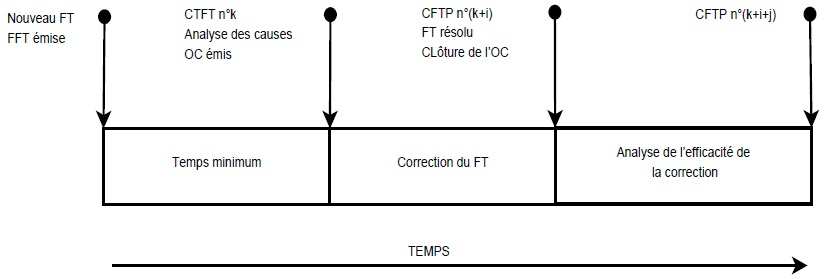
\includegraphics[width=13cm]{./images/cycle_d_un_fait_technique.jpg}
\end{figure}

\subsubsection*{\FTCourt{} relatifs aux documents soumis à l’approbation}
\paragraph*{} Les demandes de modification(s)/évolution(s)/correction(s) de documents soumis à approbation ne feront pas l'objet d'émission de \FTCourt{} si les dites modification(s)/évolution(s)/correction(s) ne concernent que la forme du document (orthographe, mise en page...).

\subsection{Audits internes}
\paragraph*{} Conformément à la Norme ISO 9001:2015 , des audits internes (un durant le premier semestre et un durant le second) seront menés pour évaluer le management de la Qualité au sein du PIC et déterminer si le \SMQCourt{} est conforme :
\begin{itemize}
\item aux exigences de la Norme ISO 9001:2015 ;
\item au \SMQ{} de l'Unité P3 du département \ASI ;
\item aux dispositions prises par la direction du PIC (engagements, \PQCourt , \PGCCourt).
\end{itemize}
\paragraph*{} La mise en place d'un tel audit consiste à vérifier que les dernières versions des documents
Qualité du PIC sont cohérentes et à jour ainsi qu'à effectuer une surveillance des configurations.
Toute remarque ou non-conformité fera l'objet d'une \FFTCourt .

\paragraph*{} Pour chaque audit, un enregistrement de l'audit et de ses résultats sera établi et conservé
puis une vérification sera faite dans le but de contrôler que la correction des éventuelles non-conformités a été faite dans le temps imparti.
